\section[Introdu��o]{Introdu��o}

\begin{frame}
    \frametitle{Introdu��o}
    \begin{itemize}
		\item fluxos de trabalho cient�fico: processamento e an�lise de dados de forma coordenada e integrada;
		\begin{itemize}
			\item encapsulamento de informa��es;
			\item processamento autom�tico em um fluxo de execu��o;
			\item gerenciados por um sistema;
		\end{itemize}
		\item problema: car�ncia de sistemas para execu��o de trabalhos cient�ficos;
		\begin{itemize}
			\item escalonadores simplistas;
		\end{itemize}
		\item proposta: SWEP - \emph{Smart Workflow Execution by Planning};
		\begin{itemize}
			\item planejador (\emph{CRIKEY});
			\item ambiente P2P (\emph{PeerUnit});
			\item caracter�sticas:
			\begin{itemize}
				\item m�tricas flex�veis;
				\item t�cnicas de paraleliza��o;
				\item proveni�ncia e metadados;
			\end{itemize}
		\end{itemize}
	\end{itemize}
\end{frame}


\begin{frame}
	\begin{changemargin}{-1cm}{-1cm}
	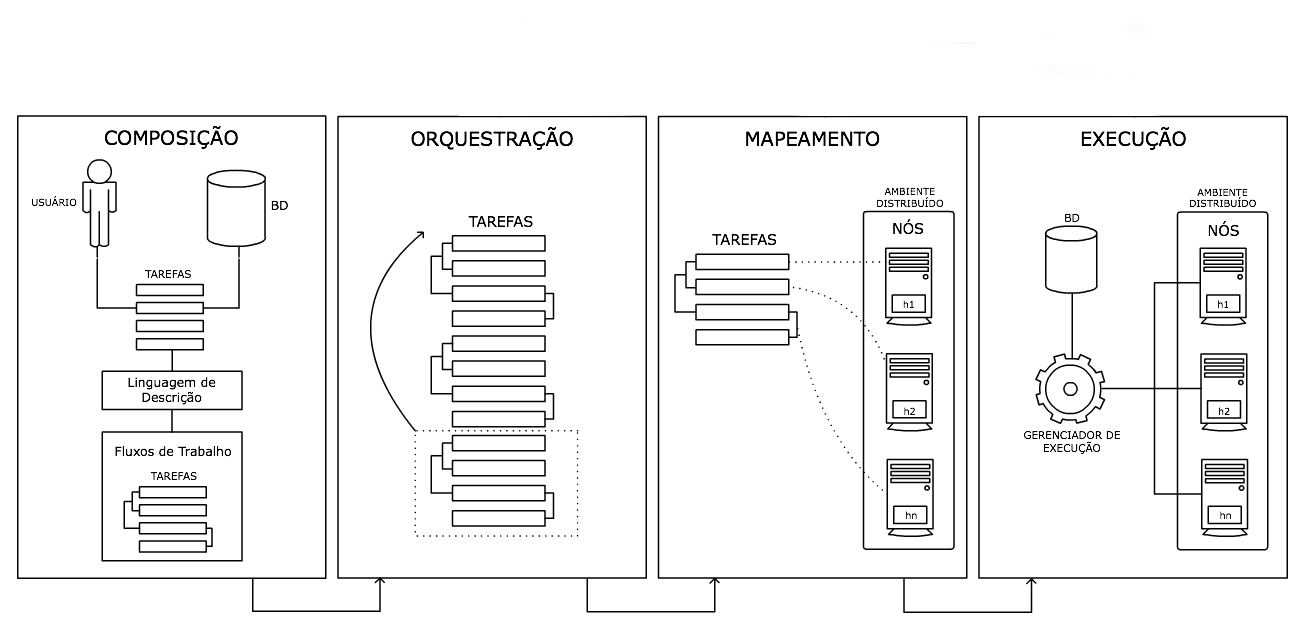
\includegraphics[width=12.8cm]{../images/fig_workflow_model_1.jpg}
	\end{changemargin}
\end{frame}

\begin{frame}
	\begin{changemargin}{-1cm}{-1cm}
	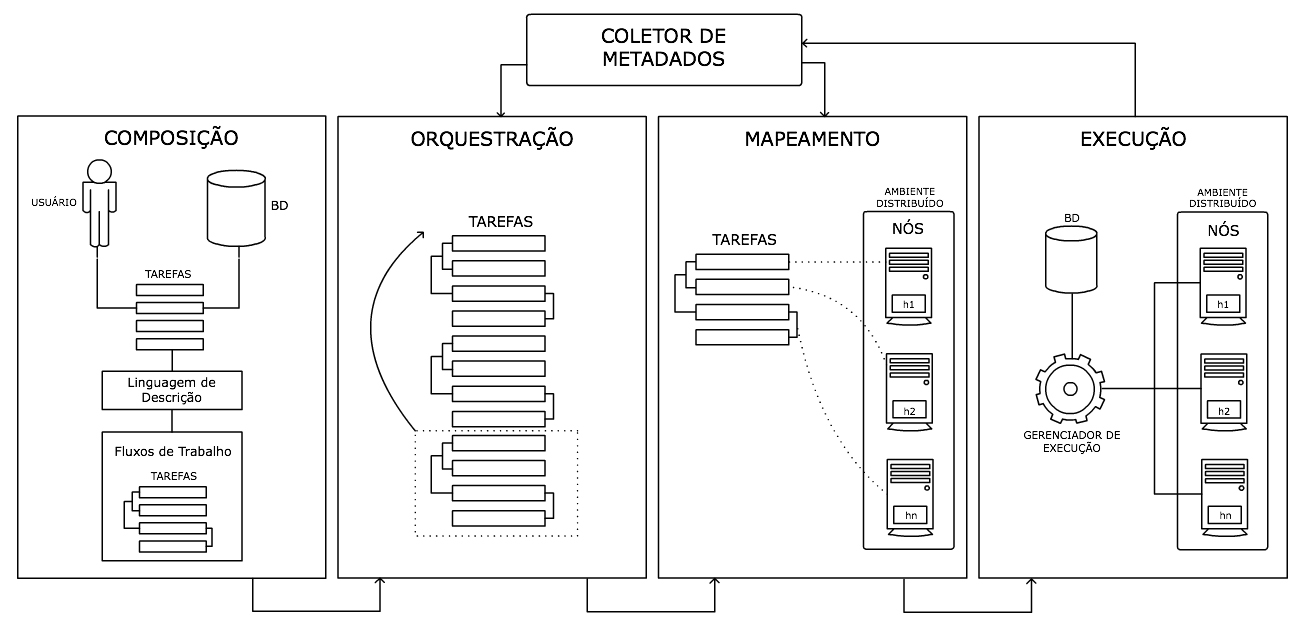
\includegraphics[width=12.8cm]{../images/fig_workflow_model_2.jpg}
	\end{changemargin}
\end{frame}

\begin{frame}
	\begin{changemargin}{-1cm}{-1cm}
	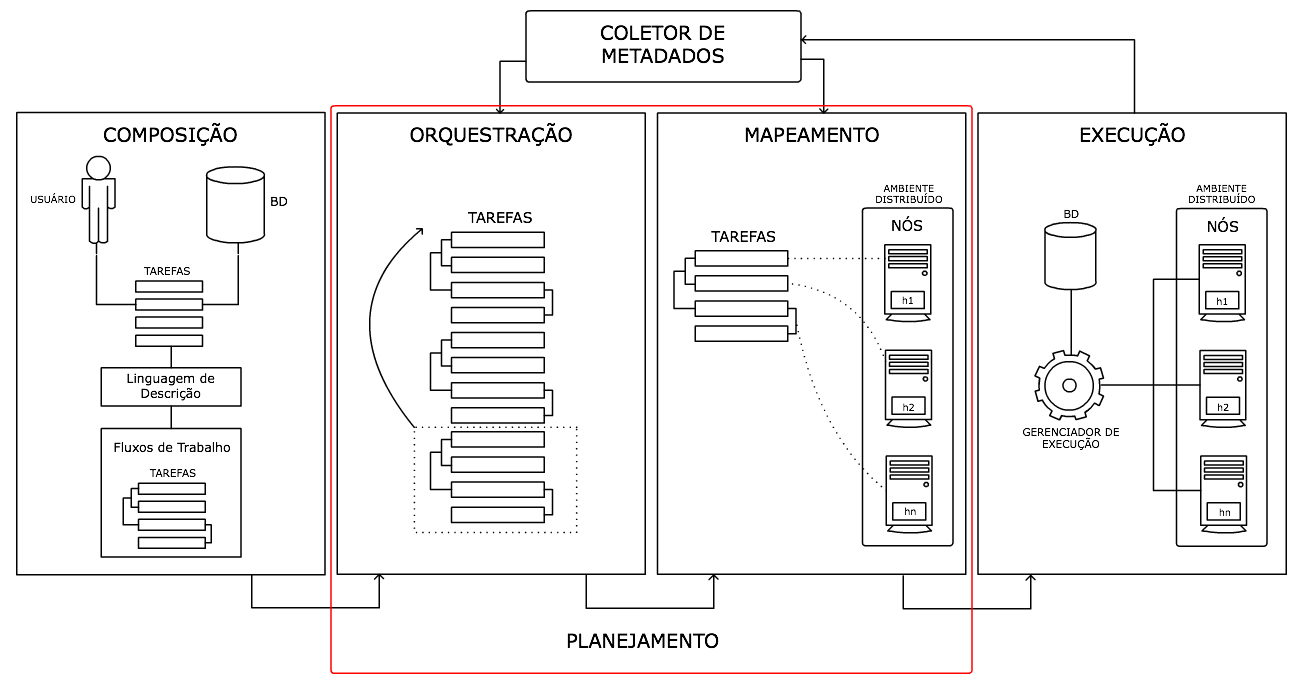
\includegraphics[width=12.8cm]{../images/fig_workflow_model_3.jpg}
	\end{changemargin}
\end{frame}